\documentclass[../main.tex]{subfile}

\tikzmath{
	%\angle = 180 - asin(2 / 3);
	\angle = 138.1896851;
}

\begin{document}

\topictitle{Conditional probability}

\begin{figure}[H]
	\centering
	\begin{minipage}{0.3\linewidth}
		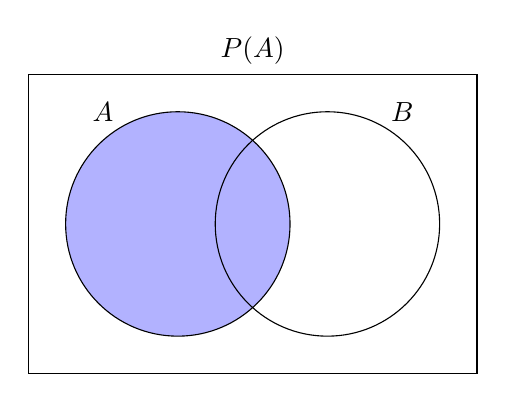
\begin{tikzpicture}[scale=0.95]
			\fill [blue!30] (-1, 0) circle[radius=1.5];

			\draw (-3, -2) rectangle (3, 2);
			\draw (-1, 0) circle[radius=1.5];
			\draw (1, 0) circle[radius=1.5];
			\node at (-2, 1.5) {$A$};
			\node at (2, 1.5) {$B$};

			\node at (0, 2) [anchor=south] {$P(A)$};
		\end{tikzpicture}
	\end{minipage}\hfill
	\begin{minipage}{0.3\linewidth}
		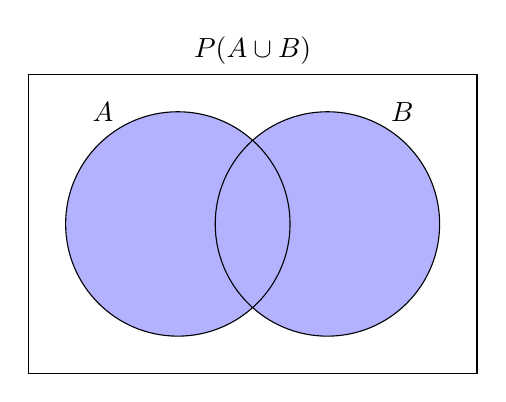
\begin{tikzpicture}[scale=0.95]
			\fill [blue!30] (-1, 0) circle[radius=1.5];
			\fill [blue!30] (1, 0) circle[radius=1.5];

			\draw (-3, -2) rectangle (3, 2);
			\draw (-1, 0) circle[radius=1.5];
			\draw (1, 0) circle[radius=1.5];
			\node at (-2, 1.5) {$A$};
			\node at (2, 1.5) {$B$};

			\node at (0, 2) [anchor=south] {$P(A \cup B)$};
		\end{tikzpicture}
	\end{minipage}\hfill
	\begin{minipage}{0.3\linewidth}
		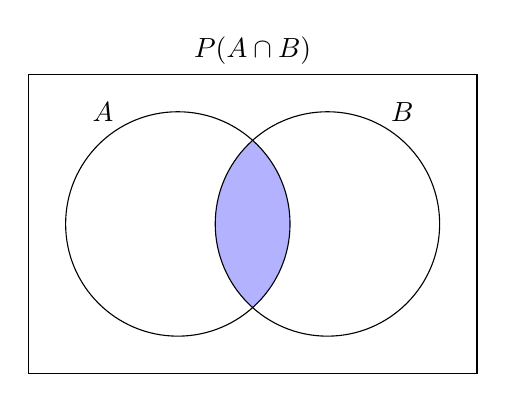
\begin{tikzpicture}[scale=0.95]
			\fill [blue!30] (-1, 0) ++(48.1896851:1.5)
				arc (48.1896851:-48.1896851:1.5)
				(1, 0) ++(228.1896851:1.5)
				arc (228.1896851:131.8103149:1.5);

			\draw (-3, -2) rectangle (3, 2);
			\draw (-1, 0) circle[radius=1.5];
			\draw (1, 0) circle[radius=1.5];
			\node at (-2, 1.5) {$A$};
			\node at (2, 1.5) {$B$};

			\node at (0, 2) [anchor=south] {$P(A \cap B)$};
		\end{tikzpicture}
	\end{minipage}
\end{figure}

\begin{figure}[H]
	\centering
	\begin{minipage}{0.3\linewidth}
		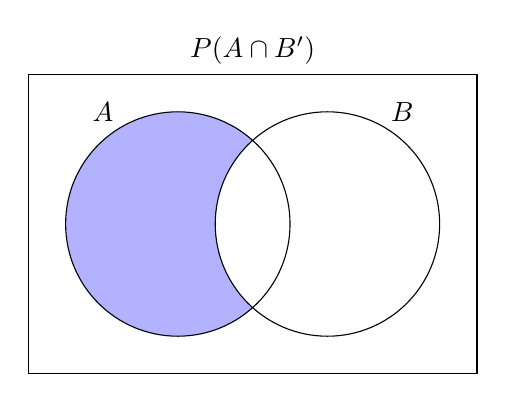
\begin{tikzpicture}[scale=0.95]
			\fill [blue!30] (-1, 0) ++(48.1896851:1.5)
				arc (48.1896851:311.8103149:1.5)
				arc (228.1896851:131.8103149:1.5);

			\draw (-3, -2) rectangle (3, 2);
			\draw (-1, 0) circle[radius=1.5];
			\draw (1, 0) circle[radius=1.5];
			\node at (-2, 1.5) {$A$};
			\node at (2, 1.5) {$B$};

			\node at (0, 2) [anchor=south] {$P(A \cap B')$};
		\end{tikzpicture}
	\end{minipage}\hfill
	\begin{minipage}{0.3\linewidth}
		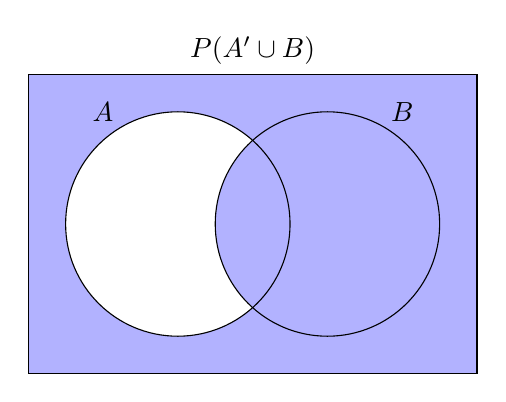
\begin{tikzpicture}[scale=0.95]
			\fill [blue!30] (-3, -2) rectangle (3, 2);
			\fill [white] (-1, 0) ++(48.1896851:1.5)
				arc (48.1896851:311.8103149:1.5)
				arc (228.1896851:131.8103149:1.5);

			\draw (-3, -2) rectangle (3, 2);
			\draw (-1, 0) circle[radius=1.5];
			\draw (1, 0) circle[radius=1.5];
			\node at (-2, 1.5) {$A$};
			\node at (2, 1.5) {$B$};

			\node at (0, 2) [anchor=south] {$P(A' \cup B)$};
		\end{tikzpicture}
	\end{minipage}\hfill
	\begin{minipage}{0.3\linewidth}
		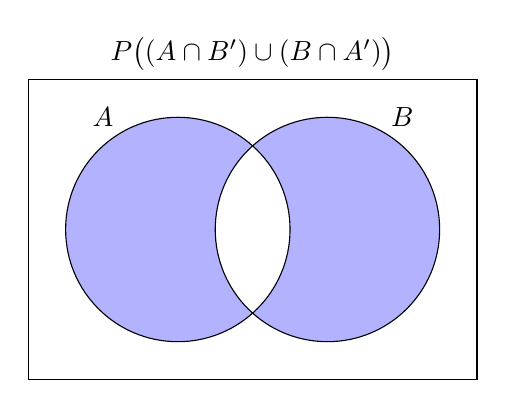
\begin{tikzpicture}[scale=0.95]
			\fill [blue!30] (-1, 0) ++(48.1896851:1.5)
				arc (48.1896851:311.8103149:1.5)
				arc (228.1896851:131.8103149:1.5);
			\fill [blue!30] (1, 0) ++(228.1896851:1.5)
				arc (-131.8103149:131.8103149:1.5)
				arc (48.1896851:-48.1896851:1.5);

			\draw (-3, -2) rectangle (3, 2);
			\draw (-1, 0) circle[radius=1.5];
			\draw (1, 0) circle[radius=1.5];
			\node at (-2, 1.5) {$A$};
			\node at (2, 1.5) {$B$};

			\node at (0, 2) [anchor=south] {$P\big((A \cap B') \cup (B \cap A')\big)$};
		\end{tikzpicture}
	\end{minipage}
\end{figure}

\begin{empheq}[box=\rememberBox]{align*}
	P(A|B) = \frac{P(A \cap B)}{P(B)}
\end{empheq}

For \underline{independent} events $A$ and $B$, we know that $P(A \cap B) = P(A) \times P(B)$. This means that $$P(A|B) = \frac{P(A \cap B)}{P(B)} = \frac{P(A) \times \cancel{P(B)}}{\cancel{P(B)}} = P(A)$$
\end{document}
